\section{Профиль и протокол}
\subsection{Цель и данные}
Цель --- проверить, даёт ли объединение аудио и видео сведения сверх ёмкости головы и как модель реагирует на пропуск и конфликт модальностей~\cite{teacher}. Использованы 1440 официальных речевых клипов RAVDESS, 24 актёра, восемь эмоций. В каждом актёре 60 клипов: четыре neutral и по восемь остальных эмоций. Единица анализа --- клип.

Актёры не пересекаются между ролями: train 14/840 клипов, val 3/180, cal 2/120, test 5/300. Применено фиксированное разбиение с seed 1729. Cal не декодируется и не участвует в признаках. На val выбираются checkpoint, стратегия и вес late fusion, test служит для итоговых оценок. В test 20 neutral и по 40 прочих классов. Основная метрика
\begin{equation}M=\frac18\sum_{c=1}^8 F1_c,\qquad F1_c=\frac{2TP_c}{2TP_c+FP_c+FN_c};\end{equation}
при отсутствующих верных ответах класса его F1 равен нулю. Accuracy --- дополнительная характеристика.

\subsection{Кодировщики и временная обработка}
Визуальный источник --- CNN из ЛР2, CIFAR ResNet-18 с выходом $d_v=512$ (R37). Кадры лица $224\times224$ извлечены с частотой 10 fps и кодируются на сетке 5 fps; ненайденные лица пропускаются, padding не входит в среднее. Полностью отсутствующих video-клипов нет. Замороженный CIFAR-кодировщик допускает размер 224 через spatial pooling, однако перенос с изображений $32\times32$ на лица является ограничением домена и масштаба.

Аудио --- mono 16 кГц. Log-mel использует 64 полосы, окно 400 отсчётов (25 мс), hop 160 (10 мс), center=True. Логарифм энергии сжимает динамический диапазон. AudioCNN имеет четыре Conv2D $3\times3$ с каналами 16,32,64,128, ReLU и pooling $(2,1)$: частота уменьшается, временной шаг остаётся 10 мс ($r=1$). AudioCNN обучена на train с остановкой по val macro-F1: максимум 100 эпох, patience 15, затем заморожена (R38). Статистики mel и pooled features рассчитаны только по train.

Время видео $\tau^v_t=t/5$, аудио $\tau^a_k=160k/16000$. Окно ширины 200 мс полуоткрыто: $-0.1\le\tau^a_k-\tau^v_t<0.1$. Границы сравниваются в целых отсчётах, av offset фиксирован метаданными. Для основной классификации используются средние валидных признаков клипа; проверка выравнивания не означает, что модель использует синхронную динамику.

\subsection{Слияние и обучение голов}
Раннее слияние конкатенирует $[z_v;z_a]$. Позднее усредняет вероятности $p_f=\lambda p_V+(1-\lambda)p_A$: обязательное $\lambda=0.5$ и выбранное по val $\lambda=0.4$ из сетки 0--1 с шагом 0.1. Нелинейная голова имеет один скрытый слой 128. Для gated общая ширина 128 и скалярный шлюз профиля:
\begin{equation}u_v=\tanh(W_vz_v),\quad u_a=\tanh(W_az_a),\quad g=\sigma(W_g[z_v;z_a]+b_g),\quad z_f=gu_v+(1-g)u_a.\end{equation}
Соглашение: $g=1$ --- видео, $g=0$ --- аудио. Кодировщики фиксированы. Головы обучаются 200 эпох, AdamW 0.001, weight decay $10^{-4}$, batch 64, CPU с двумя потоками; выбирается лучший val checkpoint без досрочной остановки головы. Признаки извлечены один раз, GPU используется для кодировщиков. Число параметров ниже относится только к обучаемой части.
\begin{figure}[H]\centering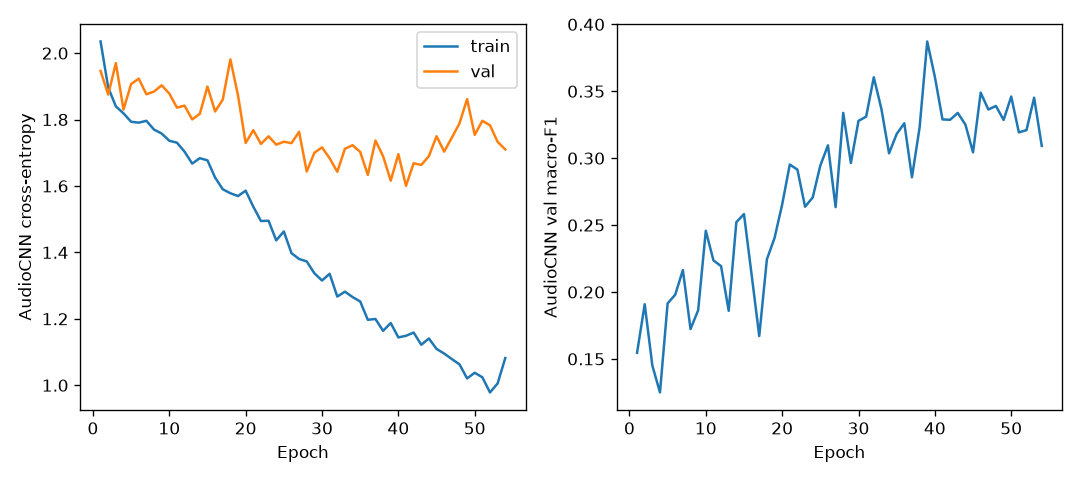
\includegraphics[width=\linewidth,height=.33\textheight,keepaspectratio]{figures/audio.png}
\caption{Обучение AudioCNN только на train, выбор по val macro-F1.}\label{fig:audio}
\end{figure}

\begin{figure}[H]\centering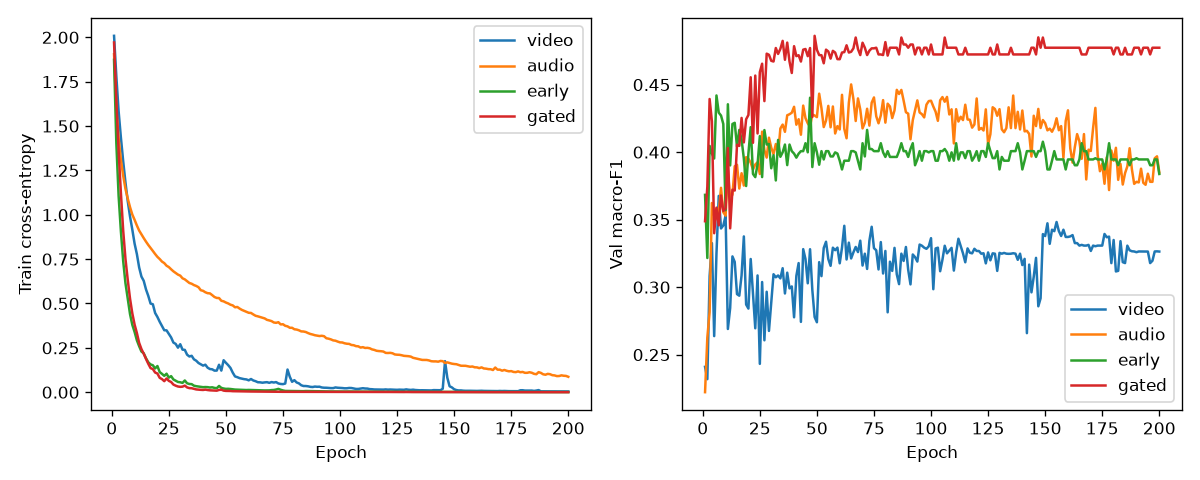
\includegraphics[width=\linewidth,height=.38\textheight,keepaspectratio]{figures/training.png}
\caption{Кривые обучения голов на сохранённых признаках.}\label{fig:training}
\end{figure}


\section{E1. Одномодальные модели и слияние}
Сначала исследованы обе одномодальные модели и три стратегии fusion. Для каждого размера fusion построены ближайшие по ширине контроли каждой модальности. Параметрический шаг равен $d_v+C+1=521$ или $d_a+C+1=137$; все фактические расхождения меньше 1\%.
\begin{table}[H]\centering\footnotesize
\setlength{\tabcolsep}{4pt}
\caption{E1: фиксированные признаки и обучаемые головы; параметры кодировщиков не включены.}\label{tab:models}
\begin{tabular}{lrrrrl}
\toprule
Модель & Val F1 & Test F1 & Accuracy & $|\theta_m|$ & Ист. \\
\midrule
Video & 0.367578 & 0.288684 & 0.306667 & 66696 & R01 \\
Audio & 0.450167 & 0.438427 & 0.456667 & 17544 & R02 \\
Early & 0.441990 & 0.488125 & 0.486667 & 83080 & R03 \\
Gated & 0.486164 & 0.509938 & 0.523333 & 100105 & R04 \\
Late 0.5 & 0.453507 & 0.456888 & 0.493333 & 84240 & R05 \\
Late val & 0.473582 & 0.450878 & 0.476667 & 84240 & R06 \\
Video+ early & 0.374748 & 0.292051 & 0.306667 & 82847 & R07 \\
Audio+ early & 0.455090 & 0.424482 & 0.440000 & 83030 & R08 \\
Video+ gated & 0.375731 & 0.321880 & 0.303333 & 100040 & R09 \\
Audio+ gated & 0.451224 & 0.416379 & 0.436667 & 100155 & R10 \\
Video+ late & 0.379016 & 0.308484 & 0.310000 & 84410 & R11 \\
Audio+ late & 0.459745 & 0.423007 & 0.440000 & 84263 & R12 \\
\bottomrule
\end{tabular}
\end{table}


\begin{figure}[H]\centering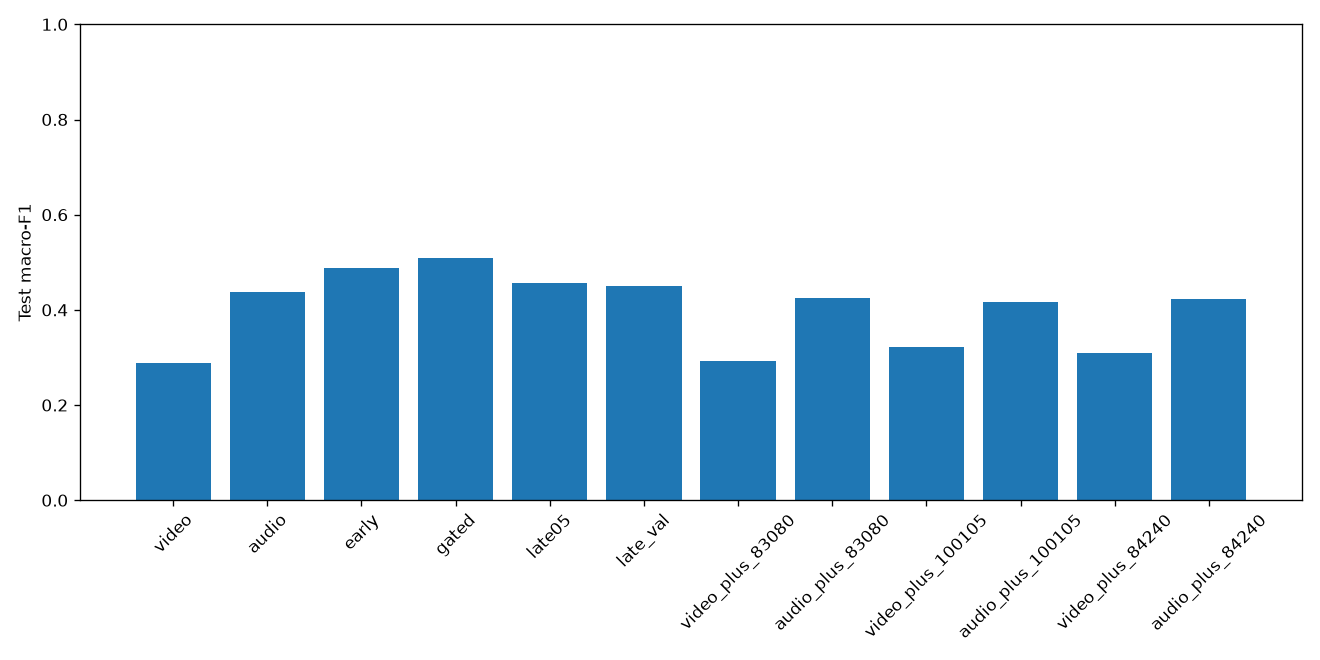
\includegraphics[width=\linewidth,height=.34\textheight,keepaspectratio]{figures/modelsfig.png}
\caption{E1: macro-F1 моделей и число обучаемых параметров.}\label{fig:modelsfig}
\end{figure}

Определены $G=M_{AV}-\max(M_V,M_A)$, $G_{ctrl}=M_{AV}-\max(M_{V^+},M_{A^+})$, $G_{int}=M_{AV}-M_{late,val}$. Late val служит ориентиром без обучаемого взаимодействия, а не доказанно оптимальным правилом fusion.
\begin{table}[H]\centering\small
\setlength{\tabcolsep}{4pt}
\caption{Исследовательские выигрыши: сравнение по одному seed, не статистическое доказательство.}\label{tab:gains}
\begin{tabular}{lrrr}
\toprule
Fusion & $G$ & $G_{int}$ & $G_{ctrl}$ \\
\midrule
Early & +0.049698 & +0.037246 & +0.063642 \\
Gated & +0.071512 & +0.059060 & +0.093560 \\
Late 0.5 & +0.018461 & +0.006009 & +0.033881 \\
Late val & +0.012452 & +0.000000 & +0.027872 \\
\bottomrule
\end{tabular}
\end{table}


\begin{figure}[H]\centering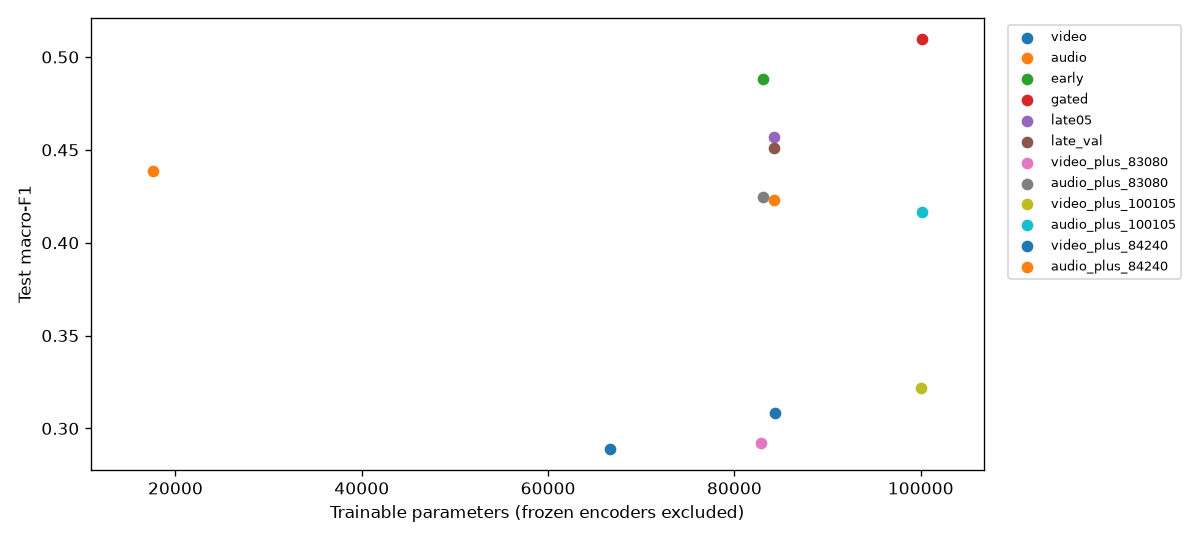
\includegraphics[width=\linewidth,height=.35\textheight,keepaspectratio]{figures/capacity.png}
\caption{Одномодальные контроли с ближайшей параметрической ёмкостью.}\label{fig:capacity}
\end{figure}

\begin{figure}[H]\centering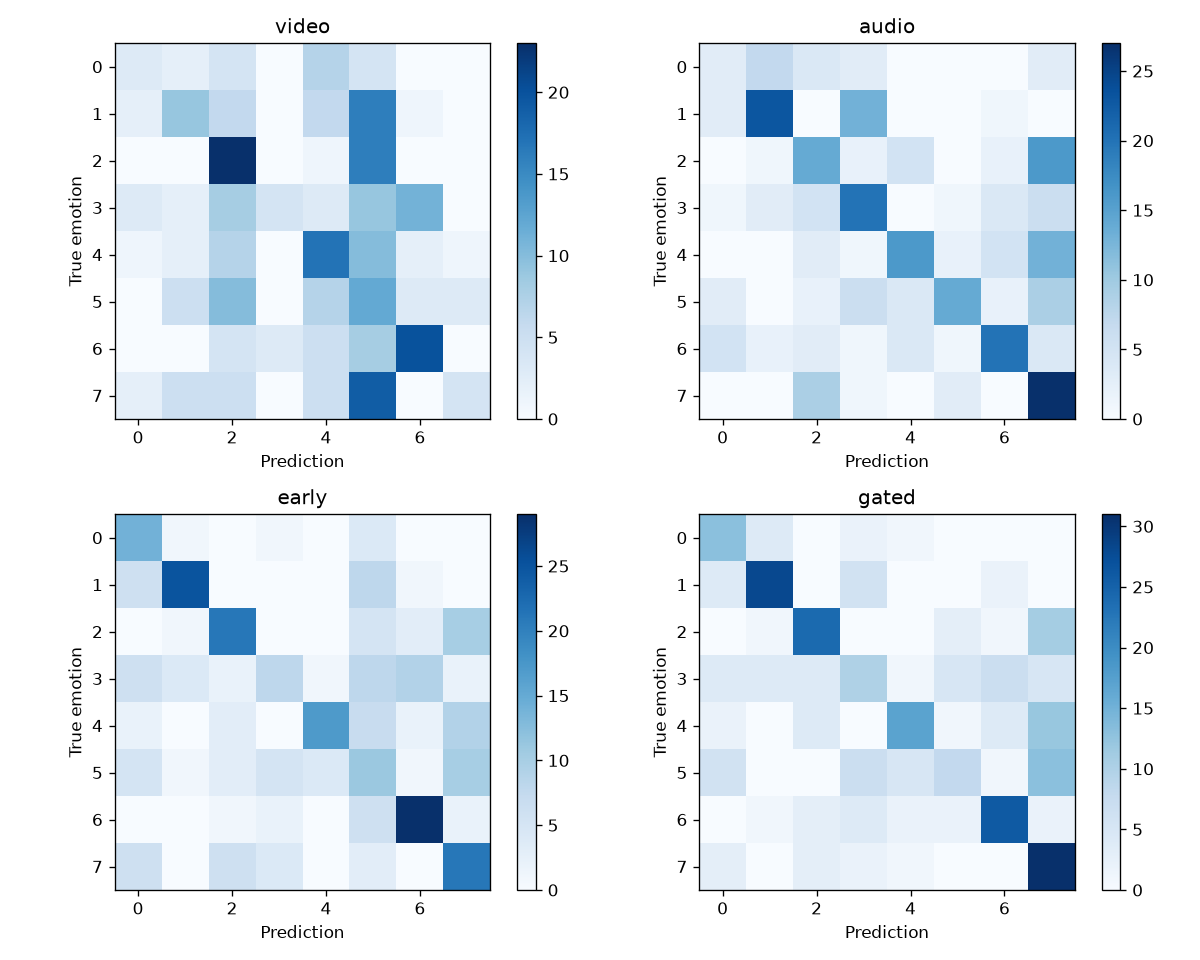
\includegraphics[width=\linewidth,height=.47\textheight,keepaspectratio]{figures/confusion.png}
\caption{Матрицы ошибок E1; единица анализа --- клип.}\label{fig:confusion}
\end{figure}

\begin{figure}[H]\centering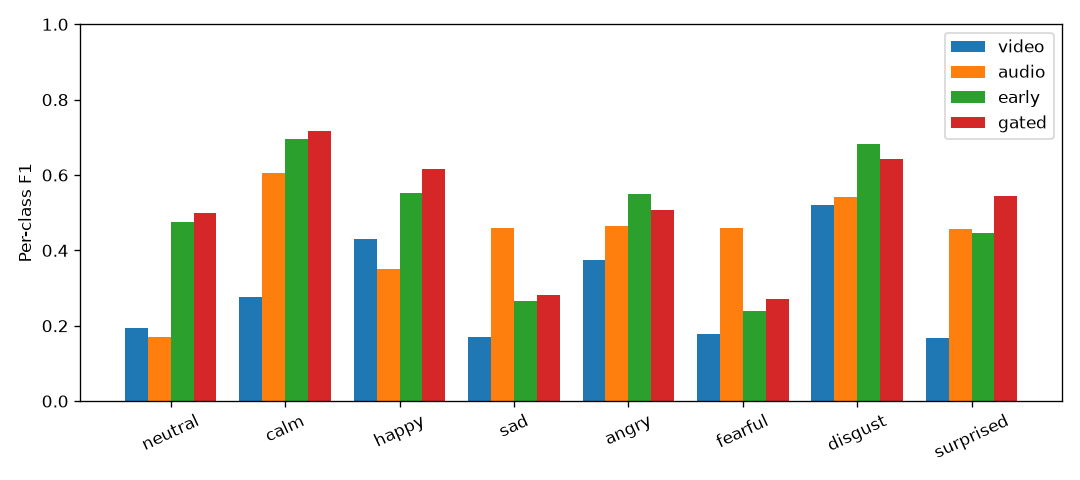
\includegraphics[width=\linewidth,height=.34\textheight,keepaspectratio]{figures/perclass.png}
\caption{Поклассовые F1 для восьми эмоций.}\label{fig:perclass}
\end{figure}

Gated выбран по val F1=0.486164, сильнейший соответствующий контроль --- audio+ ширины 731. Gated имеет 100 105 параметров, контроль 100 155, расхождение около 0.050\%. Видео-контроль имеет ширину 192 и 100 040 параметров. Простые audio/video различаются по ёмкости более чем вдвое, поэтому их разность не отделяет качество модальности от размера головы.

До основного сравнения F=Gated и U=audio+ предсказан положительный знак $\Delta_s=M_F(s)-M_U(s)$: дополнительное видео может давать комплементарные сведения. Фиксированы split, признаки, оптимизация, бюджет, правило val и близкая ёмкость. Отсутствие устойчивого положительного эффекта по правилу задания опровергло бы утверждение об установленном выигрыше. Три seed меняют инициализацию и batch голов, но не кодировщики. Все три пары заново обучены после фиксации гипотезы; исследовательский seed 1 ранее наблюдался, поэтому не объявляется новой независимой информацией.
\begin{table}[H]\centering\small
\setlength{\tabcolsep}{4pt}
\caption{Основное сравнение E1: F=Gated, U=Audio+ gated.}\label{tab:paired}
\begin{tabular}{lrrrl}
\toprule
Seed & F macro-F1 & U macro-F1 & $\Delta_s$ & Ист. F/U \\
\midrule
1 & 0.509938445 & 0.416378607 & +0.093559838 & R13/R14 \\
2 & 0.528176173 & 0.442624674 & +0.085551499 & R15/R16 \\
3 & 0.453179355 & 0.425341767 & +0.027837589 & R17/R18 \\
\bottomrule
\end{tabular}
\end{table}


\begin{figure}[H]\centering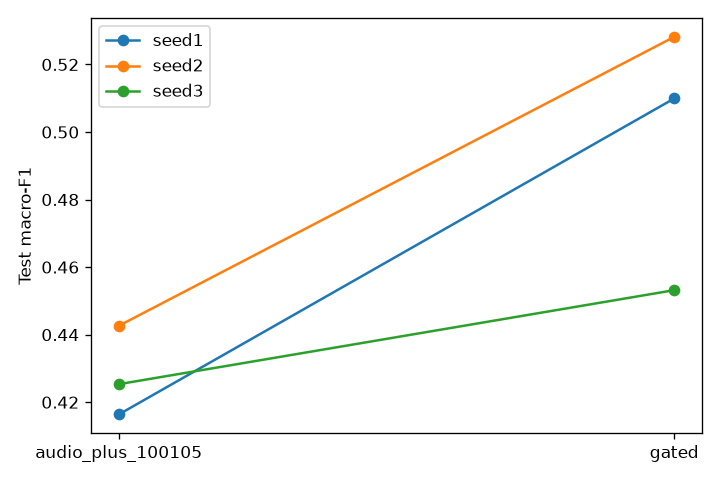
\includegraphics[width=\linewidth,height=.30\textheight,keepaspectratio]{figures/pairedfig.png}
\caption{Три положительные разности F минус U и выборочное SD; различие не установлено.}\label{fig:pairedfig}
\end{figure}

Среднее 0.068982975, выборочное SD 0.035857224. Все знаки положительны, однако $\bar\Delta<2s_\Delta=0.071714448$. Различие не установлено. Наблюдаемое направление согласуется с ожиданием, но преимущество сверх контроля по критерию преподавателя не подтверждено. Один положительный $G$ или $G_{ctrl}$ не заменяет этот вывод.

\section{E2. Пропуск и шум модальности}
Вмешательство задаётся маской $\tilde z_a=m_az_a+(1-m_a)e_a$ и аналогично для видео; $e_a=e_v=0$ в стандартизованном пространстве, одновременно обе модальности не удаляются. Для каждой фиксированной модели
\begin{equation}R_a=M_{AV}-M_{-a},\quad \tilde R_a=\frac{R_a}{M_{AV}-M_0},\quad \delta_a(x)=\|p(x)-p^{(-a)}(x)\|_1,\end{equation}
где $M_0=0.0294118$ --- наиболее частый класс; симметрично определены видео-показатели. Это вмешательство в одну модель, а не разность разных классификаторов.
\begin{table}[H]\centering\scriptsize
\setlength{\tabcolsep}{4pt}
\caption{E2: вмешательства в одну модель, нулевой заменитель, test 300 клипов.}\label{tab:missing}
\begin{tabular}{lrrrrrrrl}
\toprule
Fusion & $M_{AV}$ & $M_{-a}$ & $M_{-v}$ & $R_a$ & $R_v$ & $\tilde R_a$ & $\tilde R_v$ & Ист. \\
\midrule
Early & 0.48812 & 0.24326 & 0.33993 & 0.24486 & 0.14819 & 0.53380 & 0.32306 & R19 \\
Gated & 0.50994 & 0.23820 & 0.35209 & 0.27174 & 0.15785 & 0.56551 & 0.32849 & R20 \\
Late 0.5 & 0.45689 & 0.28868 & 0.43843 & 0.16820 & 0.01846 & 0.39348 & 0.04319 & R21 \\
Late val & 0.45088 & 0.28868 & 0.43843 & 0.16219 & 0.01245 & 0.38483 & 0.02954 & R22 \\
Gated drop & 0.43944 & 0.30555 & 0.38191 & 0.13389 & 0.05753 & 0.32654 & 0.14031 & R23 \\
\bottomrule
\end{tabular}
\end{table}


\begin{figure}[H]\centering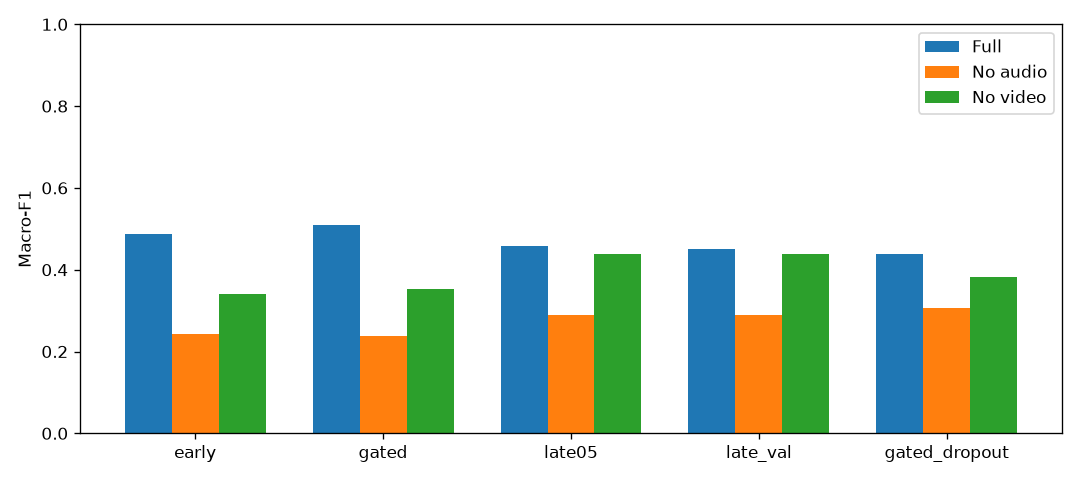
\includegraphics[width=\linewidth,height=.34\textheight,keepaspectratio]{figures/missingfig.png}
\caption{E2: полные пары, без аудио, без видео; отдельная модель с dropout.}\label{fig:missingfig}
\end{figure}

Для Gated $R_v-R_a=-0.113896$, тогда как отдельно обученные $M_V-M_A=-0.149743$. Эти разности не обязаны совпадать: разнятся архитектуры, обучение и эффект нулевого входа. Dropout с $p_{drop}=0.5$ сохраняет полную пару с вероятностью 0.5 и удаляет каждую модальность с вероятностью 0.25. В этом seed он повышает F1 без аудио с 0.238197 до 0.305552 и без видео с 0.352093 до 0.381911, но снижает полный F1 с 0.509938 до 0.439444. Это компромисс одного seed, не установленное общее преимущество.

Перестановка аудио без неподвижных точек (seed запуска 1, перестановка сохранена) даёт Gated F1=0.187489 (R39). Средний L1-эффект shuffle=1.354553 против zero mask=1.157492, доли смены класса 0.683333 и 0.620000. Значит, модель зависит от аудио; два разных заменителя не обязаны давать одну оценку вклада.

К исходной волне добавлен шум с точной мощностью:\begin{equation}\gamma=\sqrt{\sum x_a^2/(10^{SNR/10}\sum\xi^2)}.\end{equation}Затем mel и признаки заново рассчитаны тем же AudioCNN. Это искажение сигнала, не добавление шума к готовому вектору.
\begin{table}[H]\centering\footnotesize
\setlength{\tabcolsep}{4pt}
\caption{SNR по мощности исходной волны; g=1 означает видео.}\label{tab:noise}
\begin{tabular}{rrrrrl}
\toprule
SNR, dB & Gated F1 & $\bar g$ & Drop F1 & $\bar g_{drop}$ & Ист. / drop \\
\midrule
30 & 0.242099 & 0.512415 & 0.302544 & 0.590143 & R24/R25 \\
20 & 0.202144 & 0.394448 & 0.309845 & 0.654320 & R26/R27 \\
10 & 0.139632 & 0.175207 & 0.279502 & 0.679308 & R28/R29 \\
0 & 0.050072 & 0.042026 & 0.257294 & 0.674308 & R30/R31 \\
-5 & 0.035479 & 0.017611 & 0.248194 & 0.683334 & R32/R33 \\
\bottomrule
\end{tabular}
\end{table}


\begin{figure}[H]\centering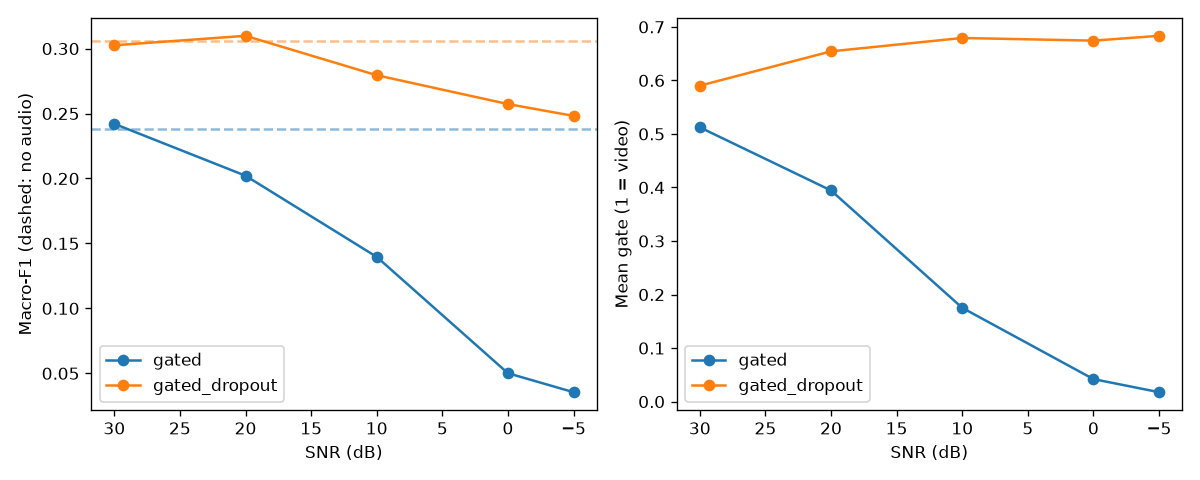
\includegraphics[width=\linewidth,height=.39\textheight,keepaspectratio]{figures/snrfig.png}
\caption{Macro-F1 и средний gate при пяти измеренных SNR.}\label{fig:snrfig}
\end{figure}

Наибольший измеренный SNR, при котором шум хуже полного удаления аудио, --- 20 дБ для Gated и 30 дБ для dropout-модели. Кривая dropout немонотонна, отличие при 30 дБ мало; это сравнение дискретных точек, не непрерывный порог. У обычной модели g уменьшается вместе с SNR, то есть смещается к шумному аудио. Dropout-модель чаще смещается к видео, но также не строго монотонно.
\begin{table}[H]\centering\footnotesize
\setlength{\tabcolsep}{4pt}
\caption{Скалярный gate на исходных test-клипах, соглашение 1=video.}\label{tab:gate}
\begin{tabular}{lrrrrrrrr}
\toprule
Эмоция & 0 & 1 & 2 & 3 & 4 & 5 & 6 & 7 \\
\midrule
$\bar g$ & 0.4675 & 0.5117 & 0.4888 & 0.5271 & 0.3345 & 0.4455 & 0.5311 & 0.4920 \\
\bottomrule
\end{tabular}
\end{table}


На исходном test средний g=0.475251, SD=0.138423; для верных/ошибочных ответов 0.474931/0.475604. Такое близкое среднее само по себе не является показателем надёжности.

\section{E3. Конфликтующие пары}
Сформированы по 300 уникальных упорядоченных пар разных актёров: A с одинаковыми эмоциями, B с разными. Seed 1 фиксирован. В A правильная метка определена; в B единого правильного класса нет. Вместо accuracy считаются доли следования видео $r_v$, аудио $r_a$ и третьему классу $r_0=1-r_v-r_a$. Для обнаружения рассогласования B --- положительный класс, A --- отрицательный; показатели $1-conf$ и эффект удаления аудио $\delta_a$ оцениваются AUROC.
\begin{table}[H]\centering\scriptsize
\setlength{\tabcolsep}{4pt}
\caption{E3: разные актёры; A --- одинаковая эмоция, B --- разные эмоции.}\label{tab:conflict}
\begin{tabular}{lrrrrrrrl}
\toprule
Fusion & A F1 & A acc. & $r_v$ & $r_a$ & $r_0$ & AUROC U & AUROC delta & Ист. \\
\midrule
Early & 0.434759 & 0.456667 & 0.173333 & 0.296667 & 0.530000 & 0.501611 & 0.504500 & R34 \\
Gated & 0.440716 & 0.476667 & 0.133333 & 0.340000 & 0.526667 & 0.564300 & 0.556700 & R35 \\
Late 0.5 & 0.417586 & 0.470000 & 0.136667 & 0.436667 & 0.426667 & 0.539272 & 0.590767 & R36 \\
\bottomrule
\end{tabular}
\end{table}


\begin{table}[H]\centering\footnotesize
\setlength{\tabcolsep}{4pt}
\caption{Средняя уверенность и изменение вероятностей при подмене аудио.}\label{tab:confstats}
\begin{tabular}{lrrrrrr}
\toprule
Fusion & Conf. A & Conf. B & $\delta_{ij,A}$ & $\delta_{ij,B}$ & $\bar g_A$ & $\bar g_B$ \\
\midrule
Early & 0.612918 & 0.611936 & 0.718412 & 1.037994 & n/a & n/a \\
Gated & 0.891621 & 0.858043 & 1.019965 & 1.429506 & 0.478021 & 0.470309 \\
Late 0.5 & 0.501510 & 0.474590 & 0.654309 & 0.853524 & n/a & n/a \\
\bottomrule
\end{tabular}
\end{table}


\begin{figure}[H]\centering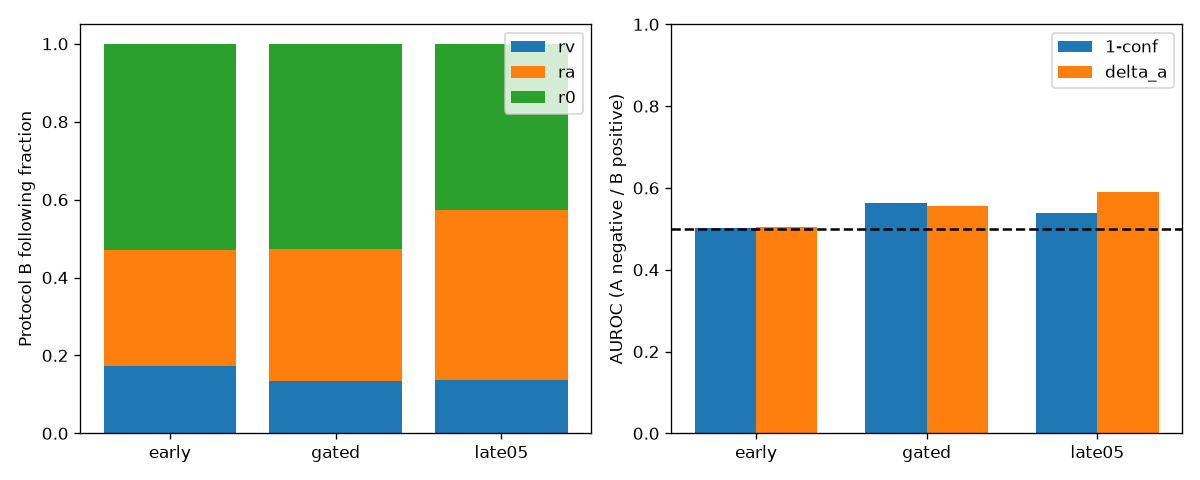
\includegraphics[width=\linewidth,height=.37\textheight,keepaspectratio]{figures/following.png}
\caption{E3: следование видео, аудио, третьему классу и обнаружение конфликта.}\label{fig:following}
\end{figure}

\begin{figure}[H]\centering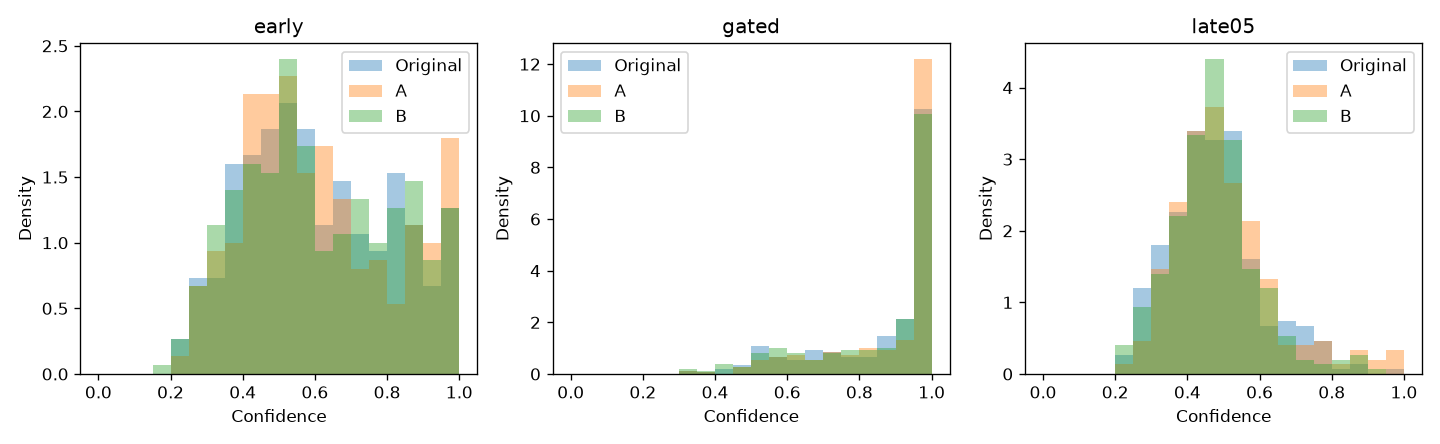
\includegraphics[width=\linewidth,height=.38\textheight,keepaspectratio]{figures/confidence.png}
\caption{Уверенность на исходных клипах, парах A и B.}\label{fig:confidence}
\end{figure}

\begin{figure}[H]\centering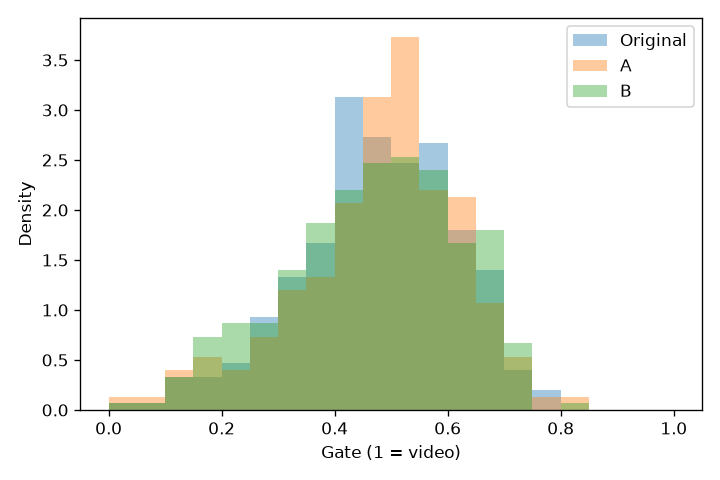
\includegraphics[width=\linewidth,height=.34\textheight,keepaspectratio]{figures/gates.png}
\caption{Gate на исходных и переставленных парах; высокое значение соответствует видео.}\label{fig:gates}
\end{figure}

Все три модели чаще следуют аудио, чем видео, но Early и Gated примерно в 53\% случаев выбирают третий класс. Поэтому «в конфликте модель всегда следует аудио» данными не подтверждается. AUROC невысок: для Gated 0.564300 по $1-conf$ и 0.556700 по $\delta_a$, близко к случайному ориентиру 0.5. Средний gate исходных пар 0.475251, A 0.478021, B 0.470309; резкого переключения не наблюдается.

На B accuracy, macro-F1, ECE и selective risk не определены, поскольку нет события «предсказание верно». Высокая confidence там не доказывает плохую калибровку. A контролирует смену актёра при совпадающей эмоции, однако повторное использование исходных клипов делает пары зависимыми. Их 300 не равнозначны 300 независимым актёрам.

\section{Ответы на контрфактические вопросы}
\subsection*{Вопрос 1. Использование слабой модальности}
Отдельная audio-модель сильнее video: 0.438427 против 0.288684. Это не обязывает fusion использовать слабое видео. В собственной Gated $\tilde R_a=0.565508$, $\tilde R_v=0.328485$, средние $\delta_a=1.157492$, $\delta_v=0.876780$. Удаление видео снижает F1 на 0.157846: зависимость вероятностей и потеря качества наблюдаются. Вывод ограничен zero-вмешательством; зависимость не равна доказанной причинной полезности во всех условиях.
\subsection*{Вопрос 2. Двойная ширина контроля}
Сохранённый контроль audio действительно переобучен 200 эпох с шириной $731\to1462$ (R40). Его F1 изменился 0.416379 $\to$ 0.406640. Новый $G_{ctrl}=0.103299$ против прежних 0.093560, изменение +0.009739. Положительное направление сохранилось в одном дополнительном seed; оно не отменяет неустановленный трёхseedовый основной результат. Дополнительная ёмкость сама по себе не гарантирует улучшения на 840 train-клипах.
\subsection*{Вопрос 3. Перемешивание и маскирование}
Почти нулевой shuffle-эффект означал бы слабую зависимость от аудио, но в наших данных он велик: L1=1.354553, смена класса 68.33\%. Маска даёт 1.157492 и 62.00\%, $R_a=0.271742$. Подмена чужим реальным аудио и нулевой вектор --- разные интервенции; чужое аудио несёт конкретный, иногда противоречащий класс, тогда как zero может быть необычным входом.
\subsection*{Вопрос 4. Размытие видео}
К исходным face-кадрам применено размытие уровня 1 сохранённого протокола, sigma 0.5, kernel 5; кадры повторно закодированы (R41). F1 упал с 0.509938 до 0.354929, g изменился лишь с 0.475251 до 0.476391. После размытия $R_v=0.002837$, средний $\delta_v=0.801904$. Даже неизменный F1 не доказывал бы устойчивости: нужно отличить сохранение полезной визуальной информации от её игнорирования. Здесь падение реально, а почти неизменный g его не отразил.
\subsection*{Вопрос 5. Должен ли gate отвергать шум}
Таблица SNR показывает противоположные реакции моделей: у обычной g падает от 0.512415 при 30 дБ до 0.017611 при $-5$ дБ, то есть вес аудио растёт. У dropout-модели g в этих точках растёт от 0.590143 до 0.683334 с немонотонными промежуточными изменениями. Обучение на чистых парах минимизирует ошибку эмоции, а не обучает детектор качества аудио. Нулевой пропуск и шумная волна тоже не одно и то же. Монотонная реакция из формулы sigmoid не следует.

\section{Ограничения и выводы}
Использован один split с пятью test-актёрами; три seed меняют только головы. Перенос CIFAR CNN на лица ограничивает обобщение. В E3 согласованность смешана с идентичностью и составом эмоций, поэтому AUROC описателен. Zero-вмешательства зависят от заменителя; изменения вероятностей не равны причинной важности.

Fusion повысил F1 относительно простых одномодальных моделей, но выигрыш над контролем той же ёмкости не установлен. Dropout улучшил обработку пропусков ценой полного качества. Gate не стал надёжным индикатором качества; конфликт требует отдельных метрик.
\clearpage
\renewcommand{\refname}{Список использованных источников}
\begin{thebibliography}{9}
\addcontentsline{toc}{section}{Список использованных источников}
\bibitem{teacher} Лабораторная работа 9. Multimodal Representation Learning. Audio-visual emotion recognition: fusion, missing modalities и modality reliability. Курс «Нейронные сети». Методические указания, 2026.
\end{thebibliography}
\clearpage
\section*{Приложение. Идентификация запусков}
\addcontentsline{toc}{section}{Приложение. Идентификация запусков}
\begingroup\small\setstretch{1.05}
\begin{longtable}{@{}l>{\raggedright\arraybackslash}p{3.5cm}p{10.8cm}@{}}
\caption{Полные RUN\_ID источников результатов.}\\
\toprule Код & Условие & RUN\_ID \\ \midrule \endhead
\hypertarget{R01}{R01} & E1 Video & {\fontsize{8.8}{11}\selectfont\texttt{73b7c031da6acfd09b36-3d018c3486d345a5bfbf442430be428e}} \\
\hypertarget{R02}{R02} & E1 Audio & {\fontsize{8.8}{11}\selectfont\texttt{872fb29a87d782c21051-cf1b54e8d2144cdda6e02712bcaef9bf}} \\
\hypertarget{R03}{R03} & E1 Early & {\fontsize{8.8}{11}\selectfont\texttt{05e36ac62488f7796fd6-370796fdf66a43a0adedf95d30e3e7ec}} \\
\hypertarget{R04}{R04} & E1 Gated & {\fontsize{8.8}{11}\selectfont\texttt{347c6157a20f623bbee4-d363e4726c5f48af848904756452a54e}} \\
\hypertarget{R05}{R05} & E1 Late 0.5 & {\fontsize{8.8}{11}\selectfont\texttt{6bce04d107b27fb66fc8-ba4bd30fd0654388bf9658deb27fd3af}} \\
\hypertarget{R06}{R06} & E1 Late val & {\fontsize{8.8}{11}\selectfont\texttt{e4f5de4987b4b2abe336-1f93deb10d944a25a354bce75dbbc85c}} \\
\hypertarget{R07}{R07} & E1 Video+ early & {\fontsize{8.8}{11}\selectfont\texttt{22f9948b3abb4e7644b2-4373bbba4ee44e4e8a9d1d8257447580}} \\
\hypertarget{R08}{R08} & E1 Audio+ early & {\fontsize{8.8}{11}\selectfont\texttt{747355daa60d2cc08a42-7018b6909b604f41b5dd48f0f459c1ae}} \\
\hypertarget{R09}{R09} & E1 Video+ gated & {\fontsize{8.8}{11}\selectfont\texttt{72d3e5c3ceda440965c2-8330b1637b8e41988ef1ee3046ecd911}} \\
\hypertarget{R10}{R10} & E1 Audio+ gated & {\fontsize{8.8}{11}\selectfont\texttt{e4b3f5a0c4e93bcc9098-08ab915d587344f9b4b4d15e30657a3e}} \\
\hypertarget{R11}{R11} & E1 Video+ late & {\fontsize{8.8}{11}\selectfont\texttt{8eb4311ca1c7650f5e21-3a6cc9195aa04290b33eeaa1488774f4}} \\
\hypertarget{R12}{R12} & E1 Audio+ late & {\fontsize{8.8}{11}\selectfont\texttt{af77dcffac5fbb7f9ab1-e7e966beb7934d78b0835c8f4079cf83}} \\
\hypertarget{R13}{R13} & main F s1 & {\fontsize{8.8}{11}\selectfont\texttt{5eaab7ee33e888c71fa7-fceda1ca709347878fe9090a1126afd6}} \\
\hypertarget{R14}{R14} & main U s1 & {\fontsize{8.8}{11}\selectfont\texttt{6d0bc1656002341df4e9-4eda2af5d1be4aeab430cced95c91b87}} \\
\hypertarget{R15}{R15} & main F s2 & {\fontsize{8.8}{11}\selectfont\texttt{071c6c3a878330b2e586-ef72728ed1404818bfb6d9dda97e29db}} \\
\hypertarget{R16}{R16} & main U s2 & {\fontsize{8.8}{11}\selectfont\texttt{e680333297ee1350883d-f8690e49d712401fb142404bab7178fa}} \\
\hypertarget{R17}{R17} & main F s3 & {\fontsize{8.8}{11}\selectfont\texttt{a29d0207d0691539b9fb-052d3bc061f04cbca48da4fb1d243237}} \\
\hypertarget{R18}{R18} & main U s3 & {\fontsize{8.8}{11}\selectfont\texttt{78d4d7224dc94ed76d19-fe318f92354b4fa9aab2d71e9007a865}} \\
\hypertarget{R19}{R19} & E2 Early & {\fontsize{8.8}{11}\selectfont\texttt{da815801667760cba3f0-f653366b50c04783bc48d69e65dc5308}} \\
\hypertarget{R20}{R20} & E2 Gated & {\fontsize{8.8}{11}\selectfont\texttt{5c2e15819ab203e984c5-dae3fc0aaf3b4cb69f28de679c8d7226}} \\
\hypertarget{R21}{R21} & E2 Late 0.5 & {\fontsize{8.8}{11}\selectfont\texttt{1b42bfe68b7ff9394755-75d0ae54282d486d96b30b596c0bd289}} \\
\hypertarget{R22}{R22} & E2 Late val & {\fontsize{8.8}{11}\selectfont\texttt{f72622bc263024125579-3642aca850794e0aae3c4a14fb0a585d}} \\
\hypertarget{R23}{R23} & E2 Gated drop & {\fontsize{8.8}{11}\selectfont\texttt{57166cbd0c7ff3e2e33f-64da840110db4d13a3e90f81c190fba6}} \\
\hypertarget{R24}{R24} & noise 30 & {\fontsize{8.8}{11}\selectfont\texttt{62cb2d053fcae434ac45-591717f25cfd44e9bdd2c69fd030d21c}} \\
\hypertarget{R25}{R25} & drop noise 30 & {\fontsize{8.8}{11}\selectfont\texttt{2094a246f6f3d4d1edc4-71d86323611f402a8148d498254c1e80}} \\
\hypertarget{R26}{R26} & noise 20 & {\fontsize{8.8}{11}\selectfont\texttt{83846d29c387fa1a0063-63cf5cfa0fca4acfacd3f08846be165a}} \\
\hypertarget{R27}{R27} & drop noise 20 & {\fontsize{8.8}{11}\selectfont\texttt{875463cbaa18bc930376-86f19dad7ac546e98298a5dfcf34c0cb}} \\
\hypertarget{R28}{R28} & noise 10 & {\fontsize{8.8}{11}\selectfont\texttt{e3556bc1cc4fa5706bd0-c427c6b42ea846378b4d650ef85fb8d9}} \\
\hypertarget{R29}{R29} & drop noise 10 & {\fontsize{8.8}{11}\selectfont\texttt{15134648de73dc39a432-33b697df06dd412d9c69e9f88970e9d6}} \\
\hypertarget{R30}{R30} & noise 0 & {\fontsize{8.8}{11}\selectfont\texttt{7cc5656e3d5ec6af2e70-d0bda4345e4e4d268d99ebef9c4adb43}} \\
\hypertarget{R31}{R31} & drop noise 0 & {\fontsize{8.8}{11}\selectfont\texttt{596dfe58808803fba854-3ed93fee76314ff48f654a8bcb3a83b6}} \\
\hypertarget{R32}{R32} & noise -5 & {\fontsize{8.8}{11}\selectfont\texttt{a219b55b3e82174a9b09-e8d748b383514f7f8e9f043155332f19}} \\
\hypertarget{R33}{R33} & drop noise -5 & {\fontsize{8.8}{11}\selectfont\texttt{a87dd8f47a24de9d1dbd-84988a0f9d2c4590a8dc369c3765f4e3}} \\
\hypertarget{R34}{R34} & E3 early & {\fontsize{8.8}{11}\selectfont\texttt{75cdef3b3621ec713c4d-8f3b5388e56e4af5b0e635d25d018b33}} \\
\hypertarget{R35}{R35} & E3 gated & {\fontsize{8.8}{11}\selectfont\texttt{bfaf1a95582bbc738bad-8f91e3804e2741cfb08e2df37488ac16}} \\
\hypertarget{R36}{R36} & E3 late05 & {\fontsize{8.8}{11}\selectfont\texttt{281261d23ef5b6ce2337-311678e304db457f8417e218a87b070e}} \\
\hypertarget{R37}{R37} & visual CNN Lab2 & {\fontsize{8.8}{11}\selectfont\texttt{cfd869bd9ae49d9e218c-674bd37aac074d9393378ce924e7c6dc}} \\
\hypertarget{R38}{R38} & AudioCNN training & {\fontsize{8.8}{11}\selectfont\texttt{1475403250d4ae591ddd-186c0d2ef7314984861ec3bcb01e4c54}} \\
\hypertarget{R39}{R39} & E2 shuffle & {\fontsize{8.8}{11}\selectfont\texttt{60613c91030bc0779023-78b0b950695a4d7cb5c3948cd630b08a}} \\
\hypertarget{R40}{R40} & CF2 double width & {\fontsize{8.8}{11}\selectfont\texttt{5d7b42d2fbe578cc1409-e0ce7e930e514b6a999d49c6b612446a}} \\
\hypertarget{R41}{R41} & CF4 blur video & {\fontsize{8.8}{11}\selectfont\texttt{975c246e6d8598e85966-8bca42f74e7d440388ce89eef547a0e0}} \\
\bottomrule\end{longtable}\endgroup
